\documentclass[12pt]{article}

\usepackage{amsmath}
\usepackage{amssymb}
\usepackage{booktabs}
\usepackage{csquotes}
\usepackage[margin=2cm]{geometry}
\usepackage{hyperref}
\usepackage{tabularx}
\usepackage{tikz}
\usetikzlibrary{patterns, shapes.geometric, positioning, bayesnet}


\title{Homework 1}

\author{CS396-4 Causal Inference}

\begin{document}

\maketitle

\section*{Instructions}

This assignment is due on Thursday, Jan 20 at 11:59pm CST. Late assignments will be accepted, but with a 14.3\% (1/7th) penalty per day late. If your assignment is less than 24 hours late, we’ll grade it and you’ll receive 85.7\% of those points; if it’s less than 48 hours late, you’ll receive 71.4\% of those points. If it’s more than 6 days late, you’ll receive no points.

Your answers must be uploaded to Canvas as a single pdf document; you should edit the LaTeX source for this pdf to add in your answers. This is an individual assignment -- you are welcome to discuss the problems with your classmates, but you must solve each part and write each answer on your own.

\subsection{(1 point)}

By submitting this assignment, you affirm that you have neither given nor received any unauthorized aid on this assignment, and that the solutions shown here are wholly you own. Any violation of \href{https://www.northwestern.edu/provost/policies/academic-integrity/index.html}{Northwestern's academic integrity policies} will result in you receiving a 0 on this assignment and a report to your dean's office. If you're ever worried about whether you are at risk of violating these policies, please ask -- we can help you follow the rules, but we can't retract a report of suspected cheating.

\clearpage

\section{Simpson's Paradox with synthetic data}

For this question, you will need to run the code provided in {\tt lecture2demo.py}. It uses the Python libraries {\tt numpy}, {\tt pandas}, and {\tt statsmodels}. If you have trouble running this code, make a post on CampusWire and we'll provide help getting set up. If you are familiar with either {\tt virtualenv} or {\tt conda}, you may find it helpful to use such an environment to manage dependencies.

\subsection{(1 point)}

Fill in the tables by running the provided code with the indicated arguments. The code returns the mean and standard deviation of {\tt repeats} samples. The first cell in each table is filled in for you. For example, in the top left table, the first cell's value is computed by running:
\begin{verbatim}
python lecture2demo.py observed --repeats 10 --c_dim 10 --ols "y ~ a"
\end{verbatim}

You will use these tables to answer the next few questions.

\begin{center}
\begin{tabularx}{\textwidth}{c c}
\centering
{
\centering
\begin{tabularx}{0.45\linewidth}{l l l}
\multicolumn{3}{c}{{\tt \bf observed(ols = "y $\sim$ a", $\ldots$)}} \\
\midrule
{\tt repeats} & {\tt c\_dim = 10} & {\tt c\_dim = 500 }\\
\midrule
10   & $-1.625 \pm 0.454$   & $26.627 \pm 73.807$  \\
100  & $-1.430 \pm 0.472$   & $36.458 \pm 66.111$  \\
1000 & $1.454 \pm 0.544$    & $29.842 \pm 71.167$     \\
\bottomrule
\end{tabularx}
}
& 
{
\centering
\begin{tabularx}{0.45\linewidth}{l l l}
\multicolumn{3}{c}{{\tt \bf observed(ols = "y $\sim$ a + c", $\ldots$)}} \\
\midrule
{\tt repeats} & {\tt c\_dim = 10} & {\tt c\_dim = 500 }\\
\midrule
10   & $0.409 \pm 0.625$  & $-0.521 \pm 5.410$  \\
100  & $0.532 \pm 0.483$  & $-0.018 \pm 3.406$  \\
1000 & $0.508 \pm 0.534$  & $ 0.508 \pm 4.286$  \\
\bottomrule
\end{tabularx}
} \\[2cm]
{
\centering
\begin{tabularx}{0.45\linewidth}{l l l}
\multicolumn{3}{c}{{\tt \bf randomized(ols = "y $\sim$ a", $\ldots$)}} \\
\midrule
{\tt repeats} & {\tt c\_dim = 10} & {\tt c\_dim = 500 }\\
\midrule
10   & $0.480 \pm 0.387$    & $-5.517 \pm 12.106$  \\
100  & $0.473 \pm 0.374$    & $1.036 \pm 14.663$   \\
1000 & $0.491 \pm 0.384$    & $0.558 \pm 14.346$   \\
\bottomrule
\end{tabularx}
}
& 
{
\centering
\begin{tabularx}{0.45\linewidth}{l l l}
\multicolumn{3}{c}{{\tt \bf randomized(ols = "y $\sim$ a + c", $\ldots$)}} \\
\midrule
{\tt repeats} & {\tt c\_dim = 10} & {\tt c\_dim = 500 }\\
\midrule
10   & $0.517 \pm 0.213$     & $0.706 \pm 1.436$    \\
100  & $0.501 \pm 0.203$     & $0.780 \pm 1.539$    \\
1000 & $0.499 \pm 0.234$     & $0.547 \pm 1.571$    \\
\bottomrule
\end{tabularx}
} \\ 
\end{tabularx}
\end{center}

\subsection{(1 point)}

The true causal effect of $A$ on $Y$ is 0.5. Which table has mean results furthest away from that value? Why?

The first table has mean results furthest away from that 0.5. This is because ...

\subsection{(1 point)}

How do the mean and standard deviation of the results change as you increase {\tt c\_dim} and {\tt repeats}? What explains these trends?

\subsection{(1 point)}

Compare the {\tt c\_dim = 500} columns in the top right table ({\tt \bf observed(ols = "y $\sim$ a + c", $\ldots$)}) and the bottom left table ({\tt \bf randomized(ols = "y $\sim$ a", $\ldots$)}). This is the only comparison (for the same value of {\tt c\_dim}) where a column in a {\tt \bf observed} table has lower variance and a mean closer to 0.5 than a {\tt \bf randomized} table. Why does this happen for this comparison? Why doesn't it happen anywhere else?

\clearpage

\section{Simpson's Paradox in expectation}

\begin{table}[!th]
\centering
\begin{tabular}{c c c}
& A=0 & A=1 \\
\midrule
C=0 & $x_1 = 0.93$ & $x_2 = 0.87$ \\
&     (81/87)        & (234/270) \\[0.5em]
C=1 & $x_3 = 0.73$ & $x_4 = 0.69$ \\
&     (192/263)      & (55/80) \\[0.5em]
Both & $x_5 = 0.78$ & $x_6 = 0.83$ \\
&     (273/350)      & (289/350) \\
\bottomrule
\end{tabular}
\caption{Simpson's Paradox, as covered in lecture. $C$ is patient age, $A$ is one of two drugs. Each cell shows average (binary) recovery rate $Y$. We've named the cells $x_i$ to make them easier to reference below.}
\label{tbl:simpsons}
\end{table}

Consider Table \ref{tbl:simpsons}, which we saw in lecture (for example, slide 9 of lecture 1).  We said that this table shows Simpson's paradox because if you don't know the causal structure of the data, you can't tell which drug ($A$ = 0 or 1) is better. If $C$ were a mediator (like a side effect), we should compare $x_5$ against $x_6$ to see which drug is best. But if $C$ were a confounder (like age), we should compare $x_1$ against $x_2$ and compare $x_3$ against $x_4$.


\subsection{(1 point)} \label{q1.1}

For $i = 1 \ldots 5$, define $x_i$ as a conditional expectation involving $Y, A,$ and $C$. For example, $x_6 = \mathbb{E}[Y \mid A=1]$.

\subsection{(1 point)}

Consider the return statement in the {\tt observed} function of {\tt lecture2demo.py}: 

{\tt smf.ols(ols, data=df).fit().params['a']}

\noindent For both {\tt ols = "y $\sim$ a"} and {\tt ols = "y $\sim$ a + c"}, write out the value returned by this line in terms of the expectations you wrote out in your answer for \ref{q1.1}.
Explain your answer based on what {\tt smf.ols} is doing.

You may assume that {\tt c\_dim = 2} and assume that $C$ is always either 0 or 1. You may find it helpful to reference the {\tt statsmodels} documentation \href{https://www.statsmodels.org/dev/generated/statsmodels.regression.linear_model.OLS.html}{here} and \href{https://www.statsmodels.org/dev/generated/statsmodels.regression.linear_model.RegressionResults.html#statsmodels.regression.linear_model.RegressionResults}{here}, as well as CampusWire post \# 9 \href{https://campuswire.com/c/GACD83E19/feed/9}{here}.

\subsection{(2 point)} \label{q:theta_and_simpsons}

Note that in Table \ref{tbl:simpsons}, $p(C=0) = 357 / 700 = 0.51$ and $p(C=1) = 343 / 700 = 0.49$. Define $\Theta = p(C=0) \cdot (x_1 - x_2) + p(C=1) \cdot (x_3 - x_4) - (x_5 - x_6)$.
What is the relationship between $\Theta$ and Simpson's Paradox? Explain.

\vspace{3cm} % Feel free to remove this additional spacing if you don't want it in your solution.

\subsection{(2 point)}

Consider the data-generating process implemented in the {\tt observed()} function in {\tt lecture2demo.py}. 
Suppose we let {\tt c\_dim = 10}; we must update our definition of $\Theta$ to include $p(C=1), p(C=2), \ldots, \text{and } p(C=10)$. 
We can also show that $\mathbb{E}[Y \mid A=1] \approx 3.055$ and $\mathbb{E}[Y \mid A=0] \approx 4.505$. 
With {\tt c\_dim} = 10 and with the new definition of $\Theta$, what is $\mathbb{E}[\Theta]$ for the {\tt observed()} data-generating process?

\subsection{(2 point)}

Let $C$, $A$, and $Y$ be binary variables where $C$ is patient age, $A$ is drug assignment, and $Y$ is recovery. Suppose we have some dataset sampled from the distribution $p(C, A, Y)$ that represents a randomized trial. Assume that $A$ is marginally randomized, such that each patient has an equal probability of receiving $A=0$ or $A=1$.
Using the definition of $\Theta$ from \ref{q:theta_and_simpsons} above, use the rules of probability to show that for this distribution, $\mathbb{E}[\Theta] = 0$.

\clearpage

\section{d-Separation in graphical models}

Consider the following DAG: 

\begin{center}
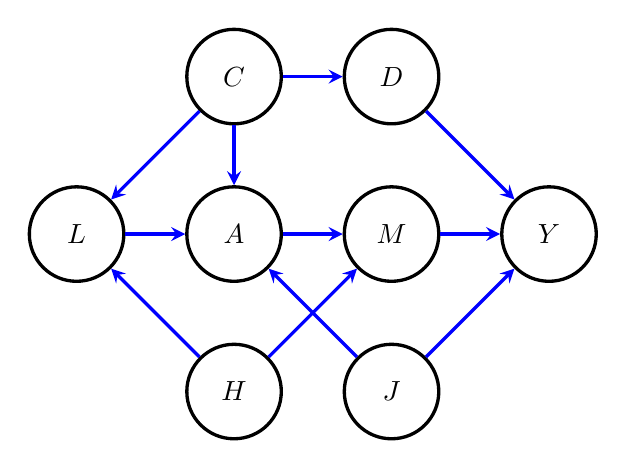
\begin{tikzpicture}[>=stealth, node distance=2cm]
    \tikzstyle{format} = [draw, very thick, circle, minimum size=1.2cm, inner sep=2pt]

    \begin{scope}
        \path[->, very thick]
            node[format] (L) {$L$}
            node[format, right of=L] (A) {$A$}
            node[format, right of=A] (M) {$M$}
            node[format, right of=M] (Y) {$Y$}

            node[format, above of=A] (C) {$C$}
            node[format, above of=M] (D) {$D$}
            node[format, below of=A] (H) {$H$}
            node[format, below of=M] (J) {$J$}

            (L) edge[blue] (A)
            (A) edge[blue] (M)
            (M) edge[blue] (Y)

            (C) edge[blue] (L)
            (C) edge[blue] (A)
            (C) edge[blue] (D)
            (D) edge[blue] (Y)

            (H) edge[blue] (L)
            (H) edge[blue] (M)

            (J) edge[blue] (A)
            (J) edge[blue] (Y)

        ;
    \end{scope}
\end{tikzpicture}
\end{center}

\subsection{(1 point)}

List all collider (``head-to-head'') nodes in the graph. For each, list all their descendants in the graph.

\subsection{(2 points)}

For each of the following parts, we write ``Is $A \perp B \mid C$'' to mean ``Is $A$ d-separated (and therefore conditionally independent) of $B$ given $C$?'' For each question, provide your explanation in terms of blocked and unblocked paths. For example, if we asked,
``Is $L \perp D \mid C$?'' it would not be enough to say ``yes'' -- you must explain, e.g.:

\begin{displayquote}
Yes, because all paths from $L$ to $D$ go through $C$ or $Y$, and the path $L \gets C \to D$ is blocked by conditioning on $C$, the path $L \to A \gets C \to D$ is blocked by conditioning on $C$, and the path $L \to A \to M \to Y \gets D$ is blocked at $Y$, a collider.
\end{displayquote}

\begin{enumerate}
\item Is $H \perp J \mid Y$? Why?
\item Is $H \perp J \mid L$? Why?
\item Is $A \perp Y \mid J, M, C$? Why?
\item Is $L \perp Y \mid A, M, C, D$? Why?
\end{enumerate}

\end{document}
